% com-cas
% by hk, rj, January 2012

\documentclass{llncs}

%create pdf images with epstopdf not ps2pdf

%todo:

\usepackage{epsfig}
%\usepackage{graphicx}
\usepackage{amssymb}
%\usepackage{amsmath}
%\usepackage{amsfonts}

\addtolength{\textheight}{1.5cm}

\newcommand{\code}[1]{\texttt{#1}}
\raggedbottom

\begin{document}

\title{Categories as classes with mixin composition}

\author{Heinz Kredel\inst{1} and Raphael Jolly\inst{2}} 
\institute{IT-Center, University of Mannheim, Germany,
\email{kredel@rz.uni-mannheim.de,}
\and Databeans, Paris, France,
\email{raphael.jolly@free.fr}}

\maketitle

\begin{abstract} 
  The modeling of algebraic structures in a strongly typed, generic,
  object oriented computer algebra software has been presented with
  the systems JAS and ScAS. We started with the design and
  implementation of strongly typed, generic and object oriented
  polynomial algorithm libraries in Java and Scala. The libraries are
  enhanced for interactive usage with the help of the Jython and JRuby
  scripting languages. The libraries have now grown by several
  algorithm versions for greatest common divisor, squarefree
  decomposition, factorization and Gr\"obner bases computation in
  separate packages. In this paper we discuss the problem of code
  organization and algebraic structure configuration and deployment.
  In search of a possible solution we study the category concept in
  Magma and Sage and propose a novel code organization scheme using
  mixin composition. The resulting code is again strongly typed,
  generic and object oriented.
\end{abstract}

%\keywords{object oriented programming, generic type-safe library, algebraic field extensions}


\section{Introduction} %------------

To be written

\subsection{Related work} % -----------------------------------

The related work published on type systems for computer algebra or
abstract data type (ADT) approaches to computer algebra has been
summarized in \cite{JollyKredel:2010,JollyKredel:2011}.  Type-safe
design considerations in computer algebra are mostly centered around
the {\em axiom} and {\em Magma} computer algebra systems and are
described, for example in
\cite{JenksSutor:1992,Watt:2003,BosmaCannonPlayoust:1997,Stein:2005,SageWiki:2009}.
%
Further related work is mentioned in the paper as required.


\subsection{Outline} % -----------------------------------



\section{Generic, typed object oriented computer algebra software} % ----------------
\label{sec:asto}

In this section we first give an introduction into the object oriented
type systems. For more details see our earlier articles and implementations
\cite{JollyKredel:2009,JollyKredel:2010,Jolly:2010,Kredel:2000,Kredel:2008a,Kredel:2008}. %,Kredel:2006
Then we discuss the design and implementation of algebraic and
transcendental extension fields together with the modeling of real
algebraic and complex algebraic extension fields. The constructed
extension fields can be used in other algorithms on polynomials with
coefficients from such fields, for example in (parallel) Gr\"obner
base or greatest common divisor computations. Other algorithms like
polynomial factorization will however require an implemented case for
such fields. Due to space limitations we will not discuss performance,
but will give some hints on computing times and possible improvements.
We will also not be able to discuss mappings of elements between the
various extension rings and fields, as for example evaluation
homomorphisms between polynomial rings. Currently all such mappings
and their application have to be coded explicitly, but some automatic
mapping construction and convenient coercion would be desirable, at
least in scripting interpreters (for a special case see Subsection
? ): %\ref{sec:deptyp}).


\subsection{Ring elements and ring factories} %------------

The basic building blocks of the type system consists of the
interfaces \code{RingElem} and \code{RingFactory} and the classes
which implement them, see figure \ref{fig:bastype}. \code{RingElem}
defines the methods which we expect to be available on all ring
elements, for example \code{multiply()},
\code{isZERO()} or \code{isUnit()} with the obvious meanings. The
construction of ring elements is done by factories, modeled after the
{\em abstract factory} creational design pattern \cite{Gamma:1995}.
The factory \code{RingFactory} defines the construction methods for
elements, for example \code{get\-ONE()} to create the one element from
the ring, 
%\code{from\-Integer()} to embed the natural numbers into the ring, \code{subtract()},
%\code{random()} to create a random element 
\code{parse()} to create an element from a string representation or query methods such as
\code{is\-Asso\-ciative()}. % to query if the ring is associative. 

\begin{figure}[thb]
\centering
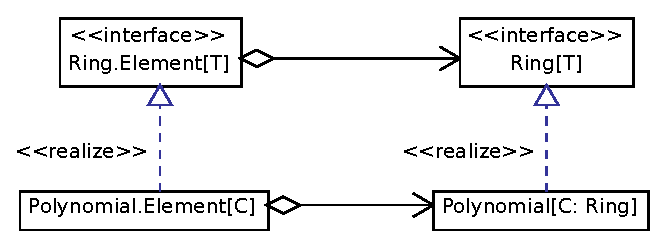
\epsfig{file=BasicTypes,clip=,width=0.7\linewidth}
%\\
\caption{Basic types}
\label{fig:bastype}
\end{figure}

The polynomial class \code{Gen\-Polynomial} with type parameter
\code{C} for the coefficient type implements the \code{Ring\-Elem}
interface and specifies that coefficients must be of type
\code{Ring\-Elem}.  In addition to the methods mandated by the
interface, the \code{Gen\-Polynomial} implements the methods like
\code{leading\-Monomial()} or \code{degree()}.  Polynomials are to be
created with a polynomial factory \code{Gen\-Polynomial\-Ring}. In
addition to the ring factory methods it defines for example methods
to create random polynomials.  The constructor for
\code{Gen\-Polynomial\-Ring} takes parameters for a factory for the
coefficients, the number of variables, the names for the variables and
a term order object \code{Term\-Order}. The relation between the
factory of the coefficients and the polynomial ring factory is modeled
after the (constructor) dependency injection pattern and implements the
inversion of control principle.

Figure \ref{fig:bastype} shows dependency arrows from the factories to
the element interfaces as factories create the respective elements.
The modeling of the constructors is not shown as it is not denotable
in Java. The constructors of ring elements implement an opposite
dependency : each constructor takes a corresponding ring
factory as parameter.  It is only indirectly enforced since the
\code{RingElem} interface specifies a method \code{factory()} to
obtain the corresponding factory.
% So methods on ring elements have access to the corresponding
% factory for construction of new elements.

The factory methods are not static (which is apparent from the
modeling as an interface) since a ring factory might depend on other
rings or specific parameters. In case of a polynomial factory it
depends on a factory for the coefficients and at least the number of
variables of the polynomial ring. By this modeling the types of
elements of algebraic structures are not simply denoted in the program
text but have to be created as programming objects (by instantiating
the respective classes). Type denotations show up explicitly in Java
program code and are mostly inferred in Scala via type resolution.

For example a polynomial $w^2 - 2 \in \mathbb{Q}[w]$ can be
constructed by first constructing an object for the ring
$\mathbb{Q}[w]$ and then reading and constructing the polynomial $w^2
- 2$ with the factory method \code{parse()}.
{\small
\begin{verbatim}
 BigRational rf = new BigRational(1); // here element = factory
 GenPolynomialRing<BigRational> pf 
  = new GenPolynomialRing<BigRational>(rf,new String[]{ "w" });
 GenPolynomial<BigRational> a = pf.parse("w^2 - 2");
\end{verbatim}
}
This example is continued in Subsection ?. %\ref{sec:anqf}.


\section{Comparison with Magma and Sage} % --------------------------------
\label{sec:magma}

In this section we discuss and compare the Magma, based on
\cite{BosmaCannonMatthews:1994,BosmaCannonPlayoust:1997}, and the
Sage, see \cite{Stein:2005,SageWiki:2009}, computer algebra systems to
our JAS and ScAS approach. We focus on the computer science aspects
and deliberately ignore performance aspects and mathematical scope of
the systems.
%
As Sage aims to provide an open source alternative to Magma
\cite{SageWiki:2009}, we first give a summary of the computer science
of mathematical concepts of Magma and then look into the Sage
implementation.

In the ``Theoretical Foundations'' of \cite{BosmaCannonPlayoust:1997}
the concepts from {\em Universal Algebra} are named as basis for the
interaction and programming language of Magma. They use order
respectively multi sorted $\Sigma$-algebras for types and provide
homomorphic images of $\Sigma$-algebras, sub-$\Sigma$-algebras,
quotient $\Sigma$-algebras and direct products of $\Sigma$-algebras.
%
However, $\Sigma$-algebras are restricted to $\Sigma$-varieties
($\Sigma$-algebras closed under sub-structure, homomorphic image and
direct product construction.
% (hence also closed under quotient structures)
Although $\Sigma$-varieties have nice mathematical properties - they
can be defined by an equational theory
%\footnote{by a theorem of Birkhoff} 
- many important algebraic structures are not
varieties. For example the class of fields (of fixed characteristic)
are not a variety because they are not closed under direct products.
So we dont see a rationale for that design decision.

$\Sigma$-algebras are then organized according to concepts from {\em
  category theory} with objects (carrier sets), morphisms, composition
of morphisms and functors between categories. Magma focuses on the
existence of free algebras (generated by some set $X$) to construct
such structures in the interaction language. The existence of
generators then allows the construction of quotients of free algebras
and the representation of homomorphisms via images of generators.

The Magma {\em computational model} starts from $\Sigma$-varieties
called {\bf magma}s $V = Var(\Sigma,P)$, where $P$ is a set of
equations over $\Sigma$. Then categories are defined as varieties
sharing the same representation $R$: $C = Cat(V,R)$. Generic functions
are modeled using abstract methods.
%examples: groups, commutative rings, modules,
Magma categories are concrete with no abstract parts of missing
implementations like {\em domain}s in Axiom and unlike the use of
categories in Axiom \cite{JenksSutor:1992}.  For example multivariate
polynomial rings indexed by coefficient rings are then modeled by
families of categories.  By the composition of categories new algebraic
structures (magmas) can be constructed. A Magma category determines
the representation of elements and the carrier sets together with the
operations on elements and carrier sets (of a magma).
%
The model then allows the creation and deletion of magmas, of elements
and morphisms, of mappings and coercion, the $\Sigma$-operations and
other representation specific operations.

The Magma {\em interaction language} is an imperative, (dynamically)
strongly typed programming language which allows algebraic structures
as first class citizens. It defines constructors for magmas and for
elements and mappings, starting from primitive (build-in) magmas.
Then the constructions from universal algebra, namely sub-structures,
quotients, homomorphisms, products and extensions are specified.
% S, Q, H, E, P universal algebra constructions
Coercions between elements of different algebraic structures are
automatic for sub-structure and quotient structures.  Coercions can
also be forced. % by the bang-notation: $type\, !\, expression$.
The Magma {\em programming language} is the same as the interaction
language. 
%
Besides loops and functions there are no ways to use object oriented
programming features, like defining classes and instantiating objects.
%
Further there is a concept to integrate and interoperate
with C programs mentioned in \cite{BosmaCannonMatthews:1994} which
seems to have disappeared in the current version of Magma.  The
integration of C programs would allow the usage of a common run-time
system with memory management and mentions some kind of interfaces
between the C parts, probably C header files.

We now look into the Sage open source implementation of Magma concepts
\cite{Stein:2005,SageWiki:2009}.  The Sage computer algebra system is
implemented in the Python scripting language \cite{vanRossum:1991}.
Python is an object oriented programming language which allows (among
many other features) hierarchical packages and can interoperate with C
libraries through Cython. Sage uses a super-set of Python in its
scripting interpreter, i.e. it provides Magma concepts together with
Python programming facilities. First there is a notable extension to
the Python syntax to allow the Magma generator assignment syntax, for
example
\begin{verbatim}
  R.<x,y> = PolynomialRing(QQ)
\end{verbatim}
This creates a multivariate polynomial ring over the rational numbers
\code{QQ} in two variables and assigns it to the (program) variable
\code{R}. Further the (program) variables \code{x} and \code{y} get
assigned the two generator polynomials of the polynomial ring. The
proposed syntax in Magma is \code{R<x,y>}, without the dot, which is
slightly different.  Without the syntax extension the example
would be
\begin{verbatim}
  R = PolynomialRing(QQ, "x,y"); (x,y) = R.gens()
\end{verbatim}
%  print x, y # -> x, y
or equivalently
\begin{verbatim}
  R = PolynomialRing(QQ, "x,y"); R.inject_variables()
\end{verbatim}
% In the jython front-end to JAS and ScAS it would be 
% \begin{verbatim}
%   R = PolyRing(QQ(), "x,y")
%   R.inject_variables()
%   print x, y # -> x, y
% \end{verbatim}
It should be noted, that the syntax extensions of Sage do not add to
the expressiveness but are solely for user convenience.

Second, the implementation of Magma concepts uses Pythons object oriented
programming features. For example the Magma categories are implemented
using abstract classes together with class (multiple) inheritance.
\begin{verbatim}
  class Category (UniqueRepresentation, SageObject):
    class ParentMethods:
    class ElementMethods:
\end{verbatim}
The \code{SageObject} class provides object serialization (called
pickling in Python) for inherited class objects. The class
\code{UniqueRepresentation} tries to ensure that such objects are
singletons, regardless of object serialization. The singletons are
maintained with the help of a Python dictionary.  The rationale for
such a design is to spare memory and uniquely identify categories by
their pointers (object references). 
%
In JAS and ScAS design we have not taken the singleton approach
because in a distributed environment, in which we envision part of the
usage, there are no singletons, except at high communication costs.
Moreover, the creation and comparison costs for the factory objects in
JAS and ScAS seem to be neglectable. The importance of object
serialization for all algebraic objects is regarded the same in JAS an
ScAS where it is ensured by implementation of the \code{Serializable}
interface.

The inner classes \code{ParentMethods} and \code{ElementMethods} are
designed to re\-cord the respective methods. For example for
(multiplicative) monoids there will be a method \code{one()} or
\code{prod()} to construct the $1$ from the category or to define the
multiplication method in \code{ParentMethods}. The element methods
class defines for example \code{is\_one()} to test if an element object
is equal to $1$ in the category.
%
Magma/Sage elements are instances of Python Sage classes and refer to
the category by the \code{parent()} method. Sage categories are using
inheritance for defining the programmatic representation properties
(such as serialization and singleton status).  The algebraic relations
between the Sage categories are maintained in a separate list of
`super categories' which are accessible via the method
\code{categories()}.  Properties of these relations are maintained
dynamically in the Python code and are not modeled using the
inheritance features or other static language features of Python.

Constructors are often designed as Python (top-level) functions, for
example for polynomial rings we have:
\begin{verbatim}
  def PolynomialRing(base_ring, names, ...):
\end{verbatim}
The parameters \code{base\_ring}, \code{names} (and others) define the
generic base ring and give names to the variables of the of the
polynomial ring.  Within the constructor function several cases, of
univariate and multivariate polynomials are distinguished and
additionally back-end polynomial objects are created. For example for
univariate polynomials an implementation of FLINT or NTL can be used
and for multivariate polynomials an implementation from Singular is
used by default.

Sage allows the user to define and implement Magma categories and
algebraic structures (magmas), which seems not possible in Magma itself.

Sage proves that categories can be designed and implemented with the
help of (partially abstract) Python classes. API interfaces, in the
sense of Java interfaces, for the Sage classes are often modeled and
maintained dynamically using inner (abstract) classes. As Sage uses
several back-end C/C++ implementations of computer algebra systems, the
Python code for methods or functions is often full of case distinctions
to level the different APIs of these systems.



\section{Mixins for software organization like categories} % -----------------
\label{sec:mixin}

An algebraic view of code organization.

Axiom: polynomial category includes for example gcd and factorization.
$\Longrightarrow$ unclear code organization and limited flexibility for
different algorithms and implementations.

is there pattern \cite{Gamma:1995} for such a use case? some kind of
simplifying facade for a complex set of classes and interfaces? or can
we sell this as a new pattern for CAS software, e.g. ``algebraic system pattern'' 



\subsection{Package structure} % -------------

Lastly, there is a question about whether several algorithm flavors
(for e.g. gcd, factorization and so on) could be implemented as
polynomial (factory) sub-classes as is currently investigated in ScAS,
or should remain in distinct class hierarchies as in JAS (see
\cite{Kredel:2008}, Subsection 7.5 ``Recursive types'').


\subsection{Implementations of different algorithms} % -------------

example several gcd implementations: different PRS, modular: Chinese
remainder or Hensel

unified by factories:
GCDFactory, SquarefreeFactory, FactorFactory, GBFactory, ...

\subsection{Polynomial GCD} % -------------

see figure \ref{fig:poly}

\begin{figure}[thb]
\centering
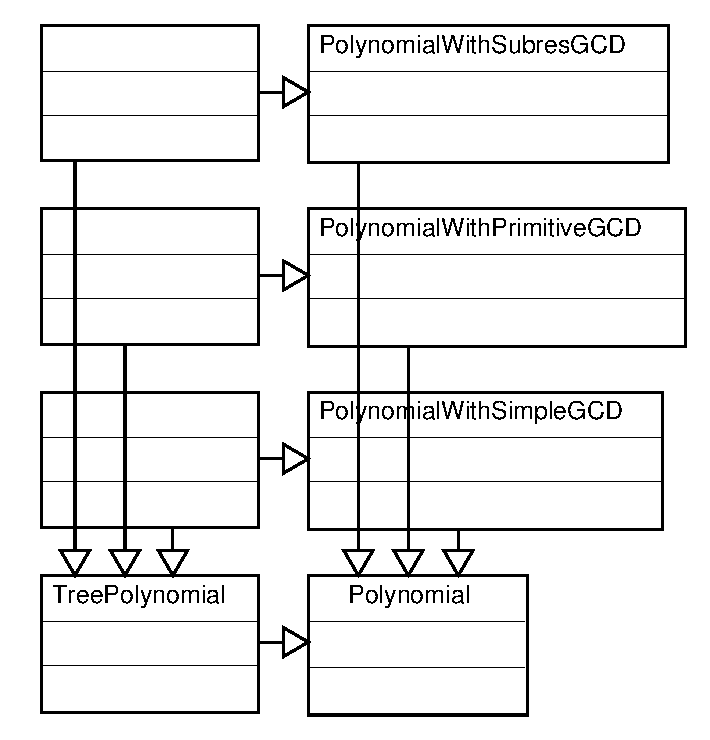
\epsfig{file=Polynomial,clip=,width=0.7\linewidth}
\caption{Polynomial GCD}
\label{fig:poly}
\end{figure}

\subsection{Categories using mixins} % -------------


\begin{verbatim}
class RationalPolynomialCategory(n: Int, vars: Array[String])
  extends PolynomialRing[BigRational](new BigRational(), n, vars)
          with GcdEngineX[BigRational] 
          with SquarefreeEngineZ[BigRational]
          with FactEngineY[BigRational]
\end{verbatim}

\begin{verbatim}
RationalPolynomialCategoryGcdXSqfZFactY
\end{verbatim}

\begin{verbatim}
trait GcdEngineX[C <: RingElem[C]] {
      //??val coFac: RingFactory[C];
      Polynomial[C] gcd(a: Polynomial[C], b: Polynomial[C]) {
                // implementation 
      }
      ...
}
\end{verbatim}

\begin{verbatim}
trait SquarefreeEngineZ[C <: RingElem[C]] {
      //??val coFac: RingFactory[C];
      Polynomial[C] squarefreePart(a: Polynomial[C]) {
                // implementation 
      }
      List[Polynomial[C]] squarefreeFactors(a: Polynomial[C]) {
                // implementation 
      }
      ...
}
\end{verbatim}

\begin{verbatim}
trait FactorEngineY[C <: RingElem[C]] {
      //??val coFac: RingFactory[C];
      List[Polynomial[C]] factorList(a: Polynomial[C]) {
                // implementation 
      }
      SortedMap[Polynomial[C],Long] factors(a: Polynomial[C]) {
                // implementation 
      }
      ...
}
\end{verbatim}

%\begin{verbatim}
%\end{verbatim}

Implementations could be retrieved via factories:
\begin{verbatim}
PolynomialCategoryFactory.<BigRational>getImplementation(coFac)
\end{verbatim}



\section{Conclusions} % --------------------------

To be written


\subsection*{Acknowledgments} %-------------------------

We thank our colleagues Thomas Becker, Wolfgang K. Seiler, Thomas
Sturm, Axel Kramer, Jaime Gutierrez, Sherm Ostrowsky, Ted Kosan and
others for various discussions on the design of and the requirements
for JAS and ScAS. 
%Thanks also to the referees for the insightful suggestions to improve the paper.


\bibliographystyle{splncs}
\bibliography{com-cas}
%\balancecolumns % insert in last page

\end{document}

%%% Local Variables:
%%% mode: latex
%%% TeX-master: t
%%% End:
